\documentclass[conference]{IEEEtran}
\usepackage{graphicx}
\usepackage{amsmath}
\usepackage{caption}
\usepackage{float}

% Title and author
\title{Performance Analysis of Pi Calculation}
\author{Charlie Flux}

\begin{document}
\maketitle

\begin{abstract}
This report examines the performance of the prefix sum algorithm while varying the number of threads
The results show the importance of parallelizable algorithms for speeding up runtimes and that deminishing returns can be found when the step count becomes large.
\end{abstract}

\section{Introduction}
The purpose of this experiment is to investigate the impace of multiple threads for execution time on calculating the prefix sum of an array using OpenMP library and the Talapas HPC. 
\section{Methodology}
Three methods for estimating pi were used:
\begin{itemize}
    \item \textbf{Sliding Window Serial $O(n^2)$:} .
    \item \textbf{Sliding Window Parallel $O(nlog(n))$:} 
    \item \textbf{Belloch Scan $O(n)$:} A parallel algorithm for computing prefix sums.
\end{itemize}

For experiments measuring time, core counts \(C\) were chosen from the set:
    \[
    C = \{1, 2, 4, 6, 8, 12, 16, 24, 32, 48, 64, 96, 128\}
    \]
with a fixed dataset size of $65536$

\subsection{Experimental Setup}
All tests were ran on Telepas. Experiments were repeated 20 times and the average was calculated for each experiment. \\
Data was filtered using the Interquartile Range Filter to remove points that do not lie between the first and third quartile as a consequence of the the unreliable data caused by the unlocked variable frequencies on Telepas.

\section{Results}
\subsection{Critical vs Atomic}
Figure~\ref{fig:prefix} compares the execution time of the sliding window and Belloch scan methods of calculating the prefix sum of an array.
\begin{figure}[H]
    \centering
    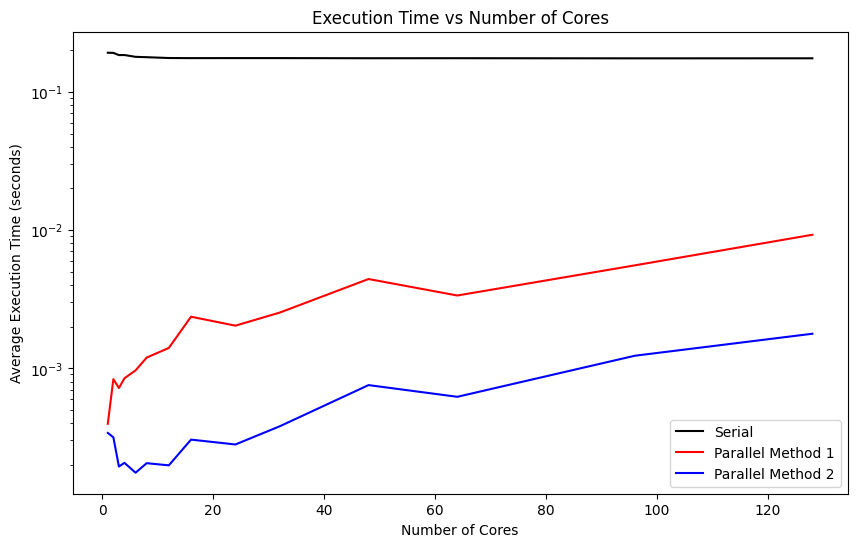
\includegraphics[width=0.45\textwidth]{../img/prefix.png}
    \caption{Sliding Window vs Belloch Scan Execution Time}
    \label{fig:prefix}
\end{figure}

\subsection{Further Speedup}
Further investigating the area of a circle code I implemented a reduction data scope on the summation of the area. \\
This removed the bottleneck that both atomic \& critical sections imposed therefore, the code now scales with more threads. \\
The increased performance of the code is seen in Figure \ref{fig:speedup} 

\begin{figure}[H]
    \centering
    \caption{Speedup using Reduction}
    \label{fig:speedup}
\end{figure}

\subsection{Comparing Speed}
Figure \ref{fig:comparingspeed} shows the performance difference of the Monte Carlo \& Area of a circle methods. Both experiments ran using reduction data scope for the inside circle counts and summation of area respectively.\\
The Monte Carlo method performs worse compared to the Area of Circle method due to the computational overhead of generating random numbers in every iteration. In contrast, the Area of Circle method relies primarily on arithmetic operations, which are efficiently handled by the ALUs, resulting in faster execution.\begin{figure}[H]

    \centering
    \caption{Accuracy with Varying Units}
    \label{fig:comparingspeed}
\end{figure}

\subsection{Comparing Accuracy}
Figure~\ref{fig:accuracy} shows the absolute percentage difference that a given estimation is to the true value of pi with a varying amount of steps that could be used.
The serial and parallel versions of the Monte Carlo method are very similar therefore, it would be safe to assume that the amount of threads given to a pi calculation does not affect the accuracy of that calculation. 
Instead the accuracy depends on the amount of guesses the Monte Carlo method has.  \\
The area of a circle method has a large advantage over the Monte Carlo method as it is using an integral approach of calculating pi instead of a random approach.

\begin{figure}[H]
    \centering
    \caption{Accuracy with Varying Units}
    \label{fig:accuracy}
\end{figure}

\section{Conclusion}
The experiments demonstrates that speedups can be found in both the Monte Carlo and Area of a Circle methods if bottlenecks are removed.
It also highlights the importance of removing bottlenecks where the cost of spawning a new thread is greater than the performance gained.
The area of a circle method sees better calculation accuracy than the Monte Carlo method due to its integral approach whereas the Monte Carlo method struggles to maintain accuracy from the randomized nature of the method.
\end{document}
